% Figure 1: measurement of endpoint agreement from one live proof state.
% Schematic only: no execution data are shown. Compile with pdflatex.
\documentclass[tikz,border=0pt]{standalone}
\usepackage[T1]{fontenc}
\usepackage[scaled=0.92]{helvet}
\renewcommand{\ttdefault}{pcr}
\renewcommand{\familydefault}{\sfdefault}
\usepackage{sansmath}
\sansmath
\usepackage{amssymb}
\usetikzlibrary{arrows.meta,positioning,calc,fit,backgrounds}
\definecolor{ink}{HTML}{1A1A1A}
\definecolor{muted}{HTML}{5C5C5C}
\definecolor{rule}{HTML}{9A9A9A}
\definecolor{accent}{HTML}{2A78D6}
\definecolor{accentfill}{HTML}{E3EEFB}
\definecolor{panel}{HTML}{F5F5F3}
\newcommand{\fs}{\fontsize{8}{9.4}\selectfont\hyphenpenalty=10000\exhyphenpenalty=10000}
% sans-serif "not equal": overlay a centred slash on the sans "=" sign
\renewcommand{\neq}{\mathrel{\ooalign{\hfil$=$\hfil\cr\hfil$/$\hfil\cr}}}
\newcommand{\fst}{\fontsize{8.2}{9.6}\selectfont}
\begin{document}
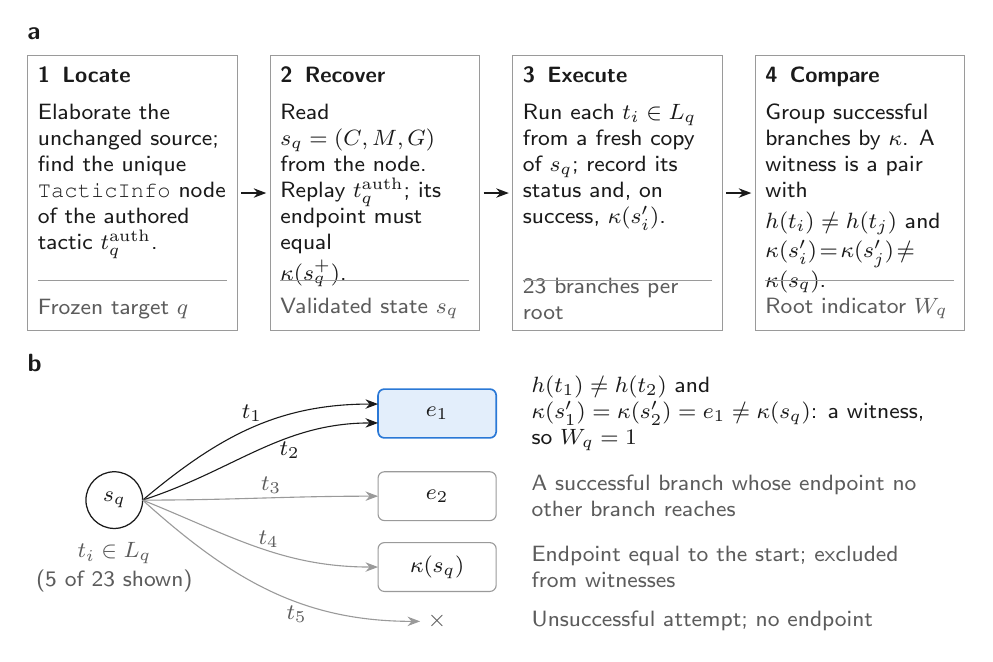
\begin{tikzpicture}[
  x=1mm,y=1mm,
  >={Stealth[length=1.6mm,width=1.2mm]},
  every node/.style={inner sep=0pt,outer sep=0pt,text=ink},
  stage/.style={draw=rule,line width=0.35pt,fill=white,minimum width=26.6mm,minimum height=35mm,anchor=north west},
  head/.style={font=\fst\bfseries,anchor=north west,text width=24mm,align=flush left},
  body/.style={font=\fs,anchor=north west,text width=24.4mm,align=flush left},
  outtxt/.style={font=\fs,anchor=south west,text width=24.4mm,align=flush left,text=muted},
  flow/.style={->,line width=0.45pt,draw=ink},
  branch/.style={->,line width=0.4pt,draw=ink},
  dimbranch/.style={->,line width=0.4pt,draw=rule},
]
% ---------------------------------------------------------------- frame
\path[use as bounding box] (0,0) rectangle (119,77);

% ---------------------------------------------------------------- panel a
\node[font=\fontsize{9.5}{11}\selectfont\bfseries,anchor=north west] at (0,77) {a};
\def\top{73.5}
\foreach \i/\x in {1/0.0,2/30.8,3/61.6,4/92.4}{
  \node[stage] (s\i) at (\x,\top) {};
}
\foreach \a/\b in {1/2,2/3,3/4}{
  \draw[flow] ($(s\a.east)+(0.5,0)$) -- ($(s\b.west)+(-0.5,0)$);
}
% stage 1
\node[head] at ($(s1.north west)+(1.3,-1.5)$) {1\enspace Locate};
\node[body] at ($(s1.north west)+(1.3,-6.2)$) {Elaborate the unchanged source; find the unique \texttt{TacticInfo} node of the authored tactic $t_q^{\mathrm{auth}}$.};
\node[outtxt] at ($(s1.south west)+(1.3,1.5)$) {Frozen target $q$};
% stage 2
\node[head] at ($(s2.north west)+(1.3,-1.5)$) {2\enspace Recover};
\node[body] at ($(s2.north west)+(1.3,-6.2)$) {Read $s_q=(C,M,G)$ from the node. Replay $t_q^{\mathrm{auth}}$; its endpoint must equal\\[0.6mm] $\kappa(s_q^{+})$.};
\node[outtxt] at ($(s2.south west)+(1.3,1.5)$) {Validated state $s_q$};
% stage 3
\node[head] at ($(s3.north west)+(1.3,-1.5)$) {3\enspace Execute};
\node[body] at ($(s3.north west)+(1.3,-6.2)$) {Run each $t_i\in L_q$ from a fresh copy of $s_q$; record its status and, on success, $\kappa(s_i')$.};
\node[outtxt] at ($(s3.south west)+(1.3,1.5)$) {23 branches per root};
% stage 4
\node[head] at ($(s4.north west)+(1.3,-1.5)$) {4\enspace Compare};
\node[body] at ($(s4.north west)+(1.3,-6.2)$) {Group successful branches by $\kappa$. A witness is a pair with\\[0.6mm] $h(t_i)\neq h(t_j)$ and\\[0.4mm] $\kappa(s_i')\!=\!\kappa(s_j')\!\neq\!\kappa(s_q)$.};
\node[outtxt] at ($(s4.south west)+(1.3,1.5)$) {Root indicator $W_q$};
\foreach \i in {1,2,3,4}{
  \draw[rule,line width=0.25pt] ($(s\i.south west)+(1.3,6.4)$) -- ($(s\i.south east)+(-1.3,6.4)$);
}

% ---------------------------------------------------------------- panel b
\node[font=\fontsize{9.5}{11}\selectfont\bfseries,anchor=north west] at (0,35.5) {b};
% start state
\node[draw=ink,line width=0.45pt,circle,minimum size=7.2mm,font=\fst] (sq) at (11,17) {$s_q$};
% endpoints
\node[draw=accent,line width=0.6pt,fill=accentfill,rounded corners=0.8mm,minimum width=15mm,minimum height=6.2mm,font=\fs,align=center] (e1) at (52,28) {$e_1$};
\node[draw=rule,line width=0.4pt,fill=white,rounded corners=0.8mm,minimum width=15mm,minimum height=6.2mm,font=\fs] (e2) at (52,17.5) {$e_2$};
\node[draw=rule,line width=0.4pt,fill=white,rounded corners=0.8mm,minimum width=15mm,minimum height=6.2mm,font=\fs] (e0) at (52,8.5) {$\kappa(s_q)$};
\node[font=\fst,text=muted] (fail) at (52,1.6) {$\times$};
% branches
\draw[branch] (sq.east) to[out=40,in=180] node[pos=0.55,above left=0.3mm and 0.1mm,font=\fs] {$t_1$} ($(e1.west)+(0,1.2)$);
\draw[branch] (sq.east) to[out=18,in=180] node[pos=0.62,below right=0.2mm and -0.6mm,font=\fs] {$t_2$} ($(e1.west)+(0,-1.2)$);
\draw[dimbranch] (sq.east) to[out=0,in=180] node[pos=0.55,above=0.5mm,font=\fs,text=muted] {$t_3$} (e2.west);
\draw[dimbranch] (sq.east) to[out=-22,in=180] node[pos=0.55,above=0.4mm,font=\fs,text=muted] {$t_4$} (e0.west);
\draw[dimbranch] (sq.east) to[out=-42,in=180] node[pos=0.6,below=0.5mm,font=\fs,text=muted] {$t_5$} ($(fail.west)+(-1,0)$);
\node[font=\fs,text=muted,anchor=north,align=center] at (11,11.6) {$t_i\in L_q$\\[0.3mm](5 of 23 shown)};
% annotations
\node[font=\fs,anchor=west,text width=52mm,align=flush left] at (64,28) {$h(t_1)\neq h(t_2)$ and $\kappa(s_1')=\kappa(s_2')=e_1\neq\kappa(s_q)$: a witness, so $W_q=1$};
\node[font=\fs,anchor=west,text width=52mm,align=flush left,text=muted] at (64,17.5) {A successful branch whose endpoint no other branch reaches};
\node[font=\fs,anchor=west,text width=52mm,align=flush left,text=muted] at (64,8.5) {Endpoint equal to the start; excluded from witnesses};
\node[font=\fs,anchor=west,text width=52mm,align=flush left,text=muted] at (64,1.6) {Unsuccessful attempt; no endpoint};
\end{tikzpicture}
\end{document}
